\chapter{实用软件}
\section{腾讯QQ}
\subsection{官方版本}
首先,我们先登录\href{https://im.qq.com/download/}{腾讯QQ官网},然后我们找到QQ Linux版,如下图~\ref{fig:download-qq}所示:

\begin{figure}[htbp]
	\centering
	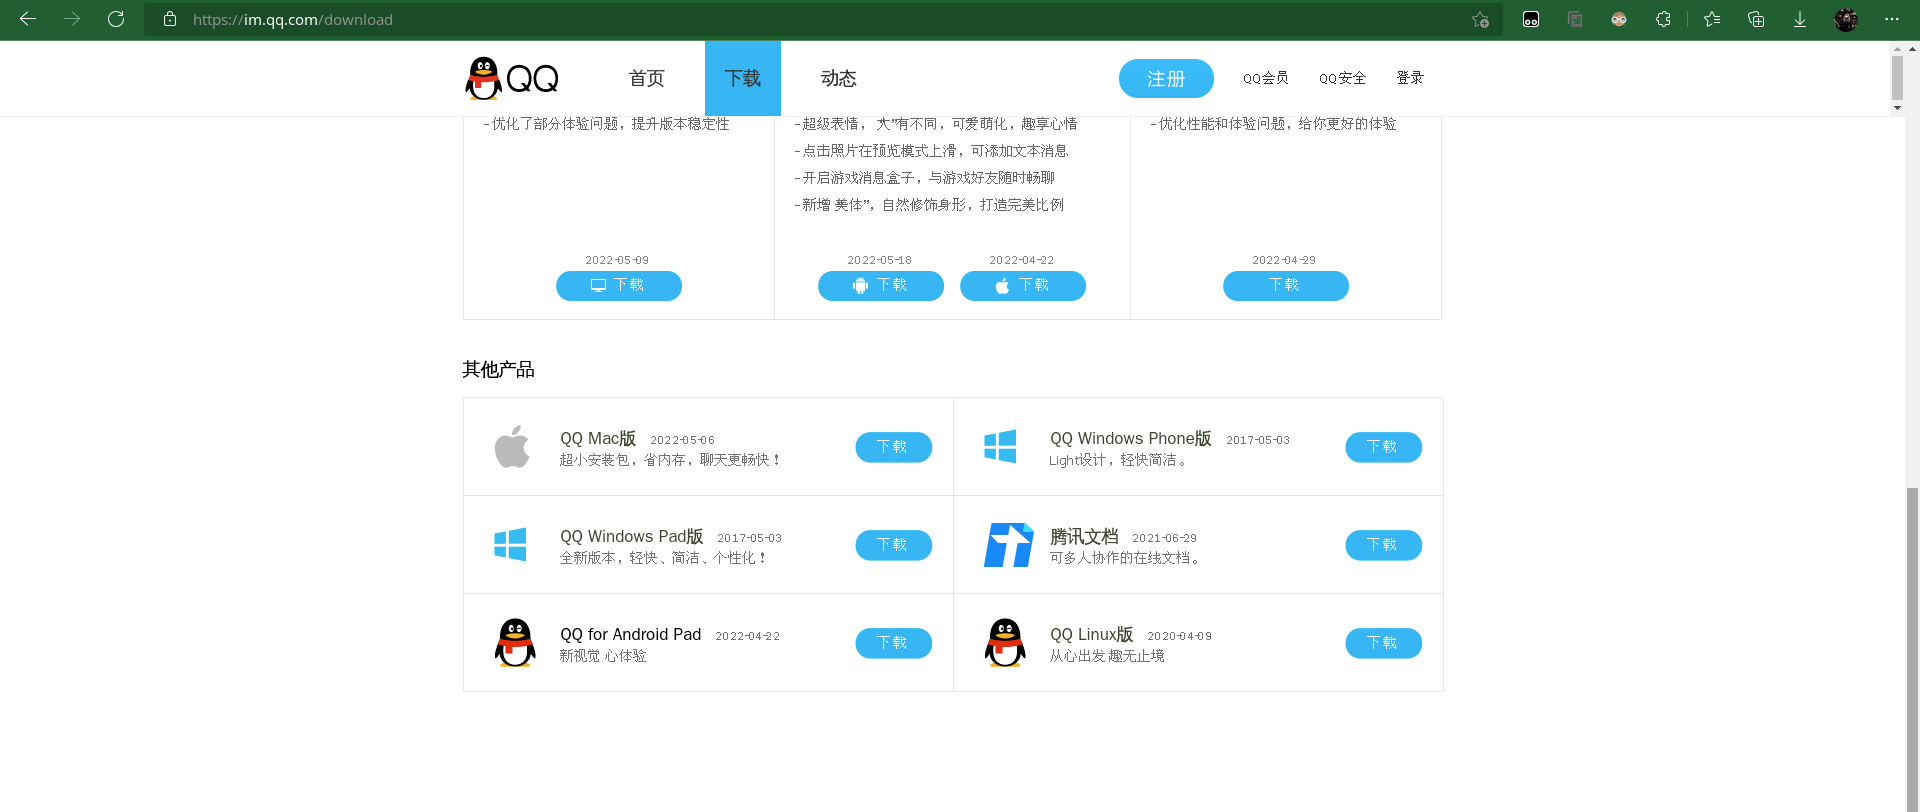
\includegraphics[width=\textwidth]{qq-download}
	\caption{QQ官网下载页}\label{fig:download-qq}
\end{figure}

如图~\ref{fig:qq-version}~选择自己合适的版本下载即可(可以使用\lstinline|uname -a|命令查看架构)
\begin{figure}[htbp]
	\centering
	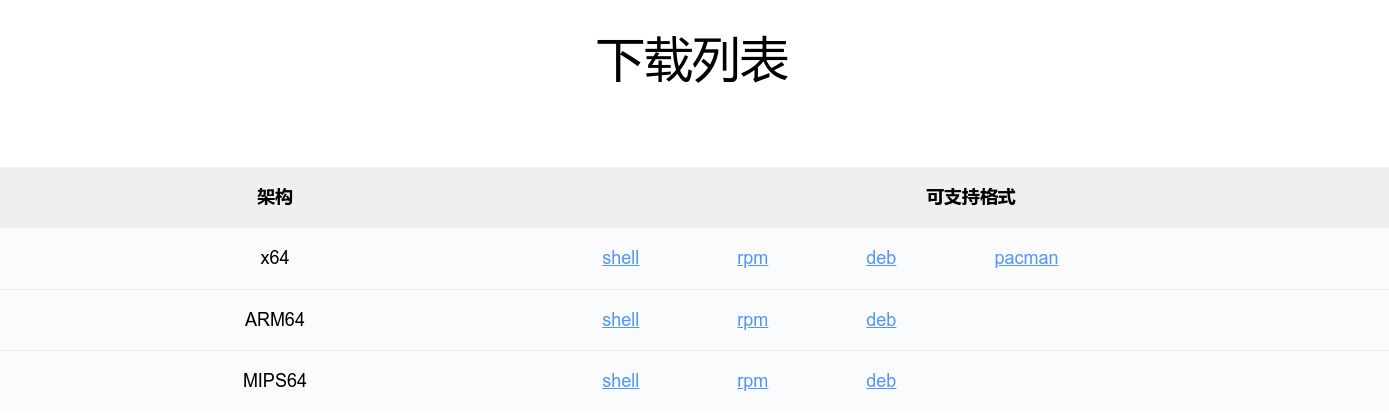
\includegraphics[width=\textwidth]{qq-version}
	\caption{QQ官网下载页}\label{fig:qq-version}
\end{figure}

下载好之后,将工作目录切换至下载的目录,使用命令
\begin{lstlisting}
sudo dpkg -i linuxqq*.deb
\end{lstlisting}
安装。安装好之后,在终端使用\lstinline|qq|命令或者在程序列表里就可以打开了。

若扫码后出现闪退的情况,可以尝试使用以下命令删除配置文件:
\begin{lstlisting}
sudo rm -rf ~/.config/tencent-qq/你的QQ号
\end{lstlisting}

\subsection{icalingua++}
Icalingua++ 是 Icalingua 的分支,为已经删除的 Icalingua 提供有限的更新。该项目希望为 Linux 打造一个会话前端框架,通过实现 Adapter 后端接口来适配各种聊天平台。目前已经拥有基于 oicq 以及 Icalingua 自有协议的后端。

\href{https://github.com/Icalingua-plus-plus/Icalingua-plus-plus}{GitHub}上可以找到最新版本,在release中可以找到对应GNU/Linux发行版的安装包或APPImage二进制文件,使用对应的命令安装使用即可。

\section{微信}
\subsection{Wine-Wechat}
\subsubsection{安装Wine}
在Debian11下安装Wine很简单,只需要一条命令即可
\begin{lstlisting}
$sudo apt-get install wine
\end{lstlisting}

安装好Wine之后,在终端输入\lstinline|winecfg|命令来对Wine进行设置
\begin{itemize}
	\item 在Application选项卡下,将Windows 版本设置为Windows10
	\begin{figure}[htbp]
		\centering
		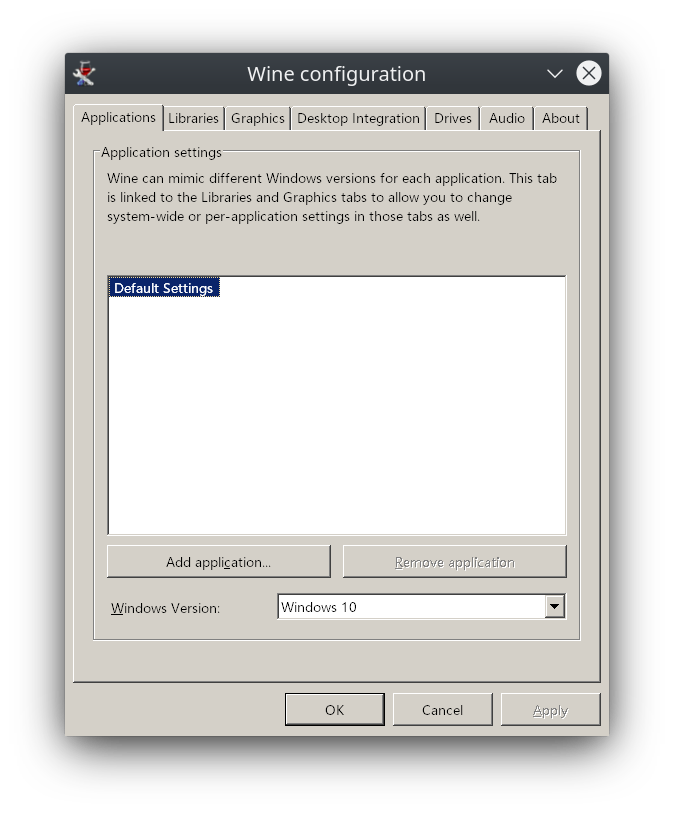
\includegraphics[height=8cm]{WindowsVersion}
		\caption{设置Windows版本}
	\end{figure}
	\item 在Graphic选项卡下,将DPI调整至120左右,较高的DPI会有一个比较好的显示效果。~图\ref{dpi}
	\begin{figure}[htbp]
		\centering
		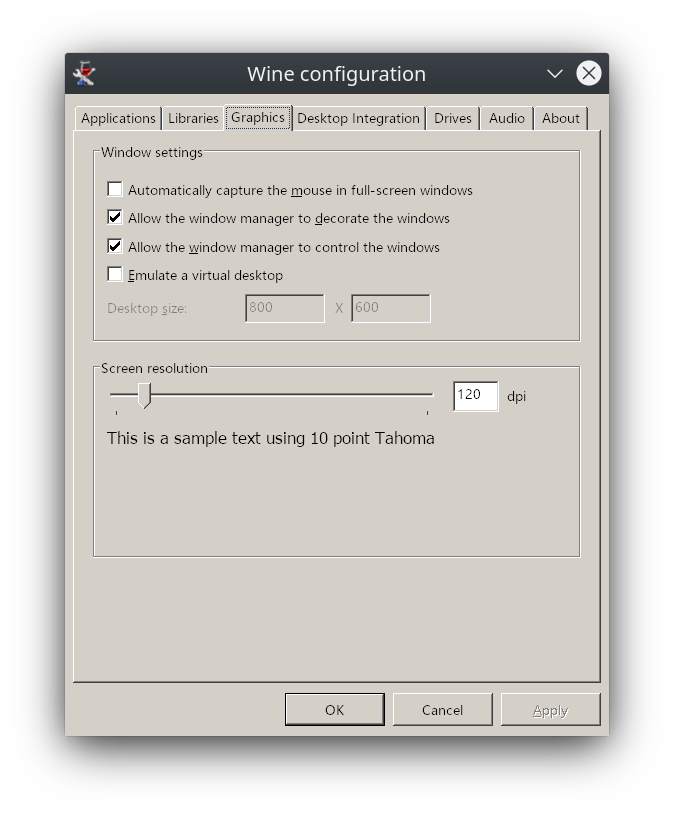
\includegraphics[height=8cm]{DPI}
		\caption{DPI设置}\label{dpi}
	\end{figure}
\end{itemize}

设置好之后,使用
\begin{lstlisting}
	wine WeChatSetup.exe
\end{lstlisting}
命令安装微信(同理,也可以使用此命令安装其他exe文件)。

安装完成之后,还需要去解决中文字体无法显示问题以及无法输入的问题。

\subsubsection{中文字体无法显示问题}
首先需要从Windows字库中获取到\lstinline|msyh.tcc|文件,拷贝到Wine的工作目录下。
\begin{lstlisting}
	cp msyh.ttc ~/.wine/drive_c/windows/Fonts
\end{lstlisting}

新建一个文本文件,保存为\verb*|font.reg|,内容如下:
\lstinputlisting{code/font.reg}

使用命令\begin{lstlisting}
	wine ~/.wine/drive_c/windows/regdit.exe font.reg
\end{lstlisting}
之后重启微信,中文就可以正常显示了。

\subsubsection{聊天框无法输入文字}
首先安装winetricks
\begin{lstlisting}
	sudo apt-get install winetricks
\end{lstlisting}
在\lstinline|~/.cache/winetricks|文件夹下,创建两个名为\lstinline|msls31|和\lstinline|win2ksp4|的文件夹,将\lstinline| InstMsiW.exe|文件放进\lstinline|msls31|目录,将\lstinline| W2KSP4_EN.EXE|文件放进\lstinline|win2ksp4|目录。

执行
\begin{lstlisting}
	winetricks riched20
\end{lstlisting}
命令,等到命令修复完成后重启微信,就可以正常使用了。


\subsection{Linux原生微信}
Linux原生的微信安装就比较简单,但原生微信是对统信UOS系统“特供”的,在安装的时候会有一个对操作系统的验证,所以需要安装一个包来把Debian系统“伪装”成国产的统信系统。用两次dpkg命令就可以安装好了。
\begin{lstlisting}
	sudo dpkg -i install-this-first.deb
	sudo dpkg -i wechat-linux-spark_2.1.2-1_amd64.deb
\end{lstlisting}
\subsection{二者对比}
其实使用起来两个都不怎么好用,Wine下的无法访问剪贴板、传输文件很麻烦;原生的实际上就是个浏览器套壳,没有时间戳、消息提示,每次登录都得扫码,用起来也很麻烦。
